\section{Setting: a calibrated market, a ring and a regulator}\label{sec:sim}

\subsection{The market and the manipulators}\label{sec:market}

\paragraph{Market.} A limit order book with price-time priority and self-trade prevention; one step is about one trading minute and a day has 240 steps. Honest agents are noise traders, market makers that re-quote two levels per side and shift with displayed depth imbalance, fundamental traders that follow a noisy latent value, capped momentum traders, depth-imbalance traders, and institutions that slice a parent order into market orders.

\paragraph{Manipulators.} A \emph{ring} of $K$ accounts (3 to 40) runs cycles of accumulation by passive buys, a push by near-simultaneous aggressive buys from several members with some cross trades, and distribution by passive sells of the stock it holds; no member sells short. Orders are spread over members; a jitter parameter spreads the members' actions in time. Outside its campaign each account trades as a noise trader. The ring's benefit is a block held beforehand (3000 lots, an assumption) and sold off-book at the end of each push, valued at the achieved price displacement, plus trading profit. Single-account spoofers, pump-and-dump agents and wash pairs are also implemented.

\paragraph{Honest groups that act in step.} A market-making firm with three to five desks that re-quote together; a fund that splits parent orders across 6 to 12 sub-accounts in the same step; and a fleet of bots that react to one public price signal with small latency differences.

\paragraph{Rules.} The exchange can apply a tick size, minimum resting time, cancel fee, circuit breaker, daily price band, and a reference-price rule for off-book blocks (the last price or a trailing mean).

\subsection{The regulator's problem}\label{sec:problem}

Let a policy $\pi=(\text{band},L,B,\text{order-level rules})$ be a choice of the daily price band, the block reference window $L$ (Section~\ref{sec:blocklaw}), the inspection capacity $B$ per window and the order-level rules. A market $\varphi$ is a draw of the honest participants (numbers and activity of noise, fundamental and momentum traders and market makers). The ring chooses a strategy $\theta$ from the set $\Theta$ of Table~\ref{tab:space} (size, orders per push, members per push, push and accumulation probabilities, jitter, cross-trade share, phase lengths) to maximise its net benefit $U(\theta;\pi,\varphi)$ of~\eqref{eq:U}; the regulator observes the ring's value $V(\pi;\varphi)=\sup_\theta U$ and the cost $C(\pi;\varphi)$ to honest participants, measured by relative changes of the spread, depth and volatility of the honest-only market. The regulator is the leader and the ring the follower of a Stackelberg game; we do not claim an equilibrium for repeated play, in which the regulator would also adapt (Section~\ref{sec:discussion}). Inspection of the $B$ top-ranked accounts uses the signed test of Section~\ref{sec:stat} on windows of 300 steps. A ring is \emph{caught} if one member is inspected in some window of the episode, on the assumption that finding one member exposes the others, as account linking does in practice, and a caught ring pays $m$ times its positive gain, with $m=5$ for individuals and $m=10$ for organisations (the caps of Vietnamese administrative fines, Appendix~\ref{app:calib}).

\begin{table}[t]
\centering\footnotesize
\begin{adjustbox}{max width=\linewidth}
\begin{tabular}{lll}
\toprule
parameter & range & meaning\\
\midrule
$K$ & 3--40 & number of ring accounts\\
$q$ & 1--6 & order size per push order (lots)\\
$m_{\mathrm{push}}$ & 1--4 & members that push together\\
$p_{\mathrm{push}},\,p_{\mathrm{acc}}$ & 0.2--1.0, 0.1--0.8 & probability that a member acts in a push step, in an accumulation step\\
jitter & 0--40 steps & spread of members' actions in time\\
cross share & 0--0.5 & share of cross trades among members\\
$\ell_{\mathrm{acc}},\ell_{\mathrm{push}},\ell_{\mathrm{dist}}$ & 20--100, 10--50, 30--80 steps & phase lengths\\
cool-down & 30--120 steps & pause between cycles\\
\bottomrule
\end{tabular}
\end{adjustbox}
\caption{Ring strategy space $\Theta$ (11 parameters).}\label{tab:space}
\end{table}

\subsection{Calibration to Vietnam}\label{sec:calib}

\paragraph{Moments.} Prices are in ticks of the Ho Chi Minh Stock Exchange (HOSE): a stock at 25,000 Vietnamese dong (VND) with a 50 VND tick has a relative tick of 20\,bp, and the daily band is $\pm 7\%$ of the previous close. Rules and statistics come from broker summaries and press (Appendix~\ref{app:calib}); the exchange rulebooks could not be fetched. We add measurements from public datasets (Table~\ref{tab:data}). Table~\ref{tab:calib} compares the first preset with the real moments. Cancel share, relative tick and daily volatility are matched; the spread (3 ticks against one tick in 73\% of futures quotes), the tails (excess kurtosis 4--5 daily and 40 at one minute) and the serial correlation of daily returns are not: simulated daily returns trend, with a lag-1 autocorrelation of 0.49 at index level and 0.60 at stock level against $-0.03$ for VN30 and 0.03 on average for HOSE stocks (Figure~\ref{fig:calibration}c). The trending comes from a slow adjustment of the price to the latent value; a family of markets in which it is calibrated away is analysed in Section~\ref{sec:acf}.

\paragraph{Index level and stock level.} The 1.16\% target is the volatility of the VN30 \emph{index} (the 30 largest HOSE stocks). A single stock is more volatile: the median HOSE stock has a daily volatility of 2.46\% since 2022, and the stocks in the enforcement cases had a median of 1.75\% in the year before the manipulation, with a share of zero-return days of 0.13 against 0.12 for HOSE stocks (Section~\ref{sec:cases}). The case stocks are therefore ordinary HOSE stocks, not unusually illiquid ones, and the daily band was reached in their manipulation periods (median five days within 0.5 points of the ceiling; one stock for 12 days in a row). We therefore build two families of calibrated markets: index level (daily volatility 0.9--1.4\%) and stock level (1.8--2.8\%).

\begin{table}[t]
\centering\footnotesize
\begin{adjustbox}{max width=\linewidth}
\begin{tabular}{p{4.2cm}p{4.3cm}p{5.2cm}}
\toprule
data & content & used for\\
\midrule
Daily prices of 1,551 Vietnamese stocks, 2015--2025 & open, high, low, close, volume & stock-level detection checks (Section~\ref{sec:real}), tick-reform experiment (Section~\ref{sec:tick}), case statistics\\
Exchange metadata & HOSE, Hanoi Stock Exchange (HNX) or Unlisted Public Company Market (UPCoM) for each ticker & control group for the tick reform; band of each case stock\\
VN30, VN-Index, VN100 bars from 2012 & daily and 30-minute bars & index-level volatility target\\
1.56 million VN30 futures ticks, 2024--25 & price, best bid and ask & spread, tick activity (not matched)\\
10 documented enforcement cases & stock, exact period, accounts, decision & weak labels for detection checks\\
701 Telegram-organised pumps & tick trades around the pump, no accounts & accumulation before pumps, early-warning limits\\
Published rules and statistics & tick, band, lot, cancel share, retail share, fine cap & simulator rules and moments\\
Order submissions of 1,909 accounts, Hyperliquid SOL perpetual, 23.6 minutes & order, account, side, time & calibration and planted ring on real accounts (Section~\ref{sec:real-accounts})\\
Fills of three Hyperliquid perpetuals, 91 minutes & account address, side, millisecond time & check of the mirror effect of executed trades\\
\bottomrule
\end{tabular}
\end{adjustbox}
\caption{Data used. Only the last two rows contain account identifiers (pseudonymous addresses on a crypto derivatives venue); no Vietnamese account-level data are used.}\label{tab:data}
\end{table}

\begin{table}[t]
\centering\footnotesize
\begin{adjustbox}{max width=\linewidth}
\begin{tabular}{lrrl}
\toprule
moment & simulator & real & source\\
\midrule
cancel share of orders & 0.321 & 0.318 & HOSE, December 2020 (press)\\
relative tick (bp) & 21 & 20 & derived from the tick table\\
daily volatility, index level (\%) & 1.14 & 1.16 & VN30, 2023 onward\\
daily volatility, typical stock (\%) & -- & 2.46 & HOSE median stock, 2022 onward\\
retail share of value & 0.72 & 0.75--0.82 & press estimates, 2024--25\\
spread: share of quotes at one tick & 0 & 0.73 & VN30F1M, 2024--25\\
lag-1 autocorrelation of daily returns & 0.49 / 0.60 & $-0.03$ / 0.03 & VN30 / mean of HOSE stocks, 2022--25\\
\bottomrule
\end{tabular}
\end{adjustbox}
\caption{Calibration of the first Vietnam preset. The last two rows are not matched; the stock-level family targets the volatility of a typical stock.}\label{tab:calib}
\end{table}

\begin{figure}[t]
\centering
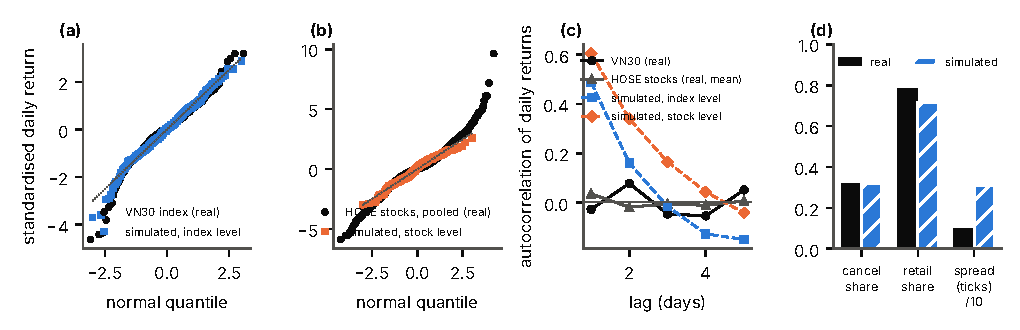
\includegraphics[width=\linewidth]{figures/calibration.pdf}
\caption{Calibration of the simulated markets against real data. (a) Standardised daily returns of the VN30 index since 2023 and of the first accepted index-level market, against normal quantiles. (b) Pooled standardised daily returns of 378 HOSE stocks since 2022 and of the first accepted stock-level market. (c) Autocorrelation of daily returns at lags 1 to 5: VN30 index, mean over HOSE stocks, and the first accepted market of each simulated family (pooled over episodes). (d) Cancel share, retail share (midpoint of the published range 0.75--0.82) and spread in ticks divided by 10 (VN30 futures: one tick for 73\% of quotes); the simulated spread is not matched}\label{fig:calibration}
\end{figure}
